\chapter{Background}
\label{chap:background}
\lhead{\emph{Background}}
%The key question to answer in this chapter is: "What has been done/is being done". 

%This chapter comprises around 4000 words and should put your project into context within Computer Science. Your focus here should be on the final section "Current State of the Art". This should be at least 2500 of the 4000 words of this section.

\section{Thematic Area within Computer Science}
While carrying out extensive research, I aim to investigate if migration can occur between single board computers while micro-services are present using containerization. To attempt to place this project within a thematic area within computer science, first, it is essential to understand the different areas that lie within the banner of computer science. Computer science is defined as "the study of theory, experimentation and engineering that forms the basis for the design and use of computers". \cite{Reference16} There are two main areas to which this area can be divided, theoretical disciplines and practical disciplines. The area to which this project scope lies is within the practical disciplines. Practical disciplines accumulates theories, methods and techniques for a specific purpose, in this case, how containerization can be used to migrate micro-services between single board computers. If all aspects are to be analyzed individually, we would see that this project falls under the headings, Complex Systems, Cloud Computing and Human Computer Interfaces. 

Complex Systems is composed of many components that interact with each other. These systems behaviours are difficult to model because of the dependencies, relationships and many other interactions which occur between parts of any given system. Internet of things falls under the scope of a complex systems. Internet of things or IOT is a system of interrelated devices. Anything which can be connected to the internet is classed as an IOT device. IOT is being used more frequently all over the world by big corporations in order to enhance their customers experiences. Single board computers are IOT devices.

Cloud Computing relies on the sharing of these resources to achieve shared pools of configurable computer system resources and high level service that can be provisioned with minimal effort. Cloud computing allows services to be scaled with ease, in turn, delivering the correct resources at the correct time while also having the freedom to expand. One aspect of cloud computing which is extremely attractive for companies is, no in-house infrastructures. With cloud computing, everything desired is stored on an external location but is easily and quickly accessible from your location. This area is the main area to which this project falls under.

Human Computer Interfaces or HCI's focus on the interfaces between people and computers. Humans interact with computers in many ways, depending on the level of understanding the individual has of computers. Graphical User Interfaces or GUI's as they are most commonly known, allow users to navigate and engage with compute systems with much more ease than without. 

\section{Project Scope}
The previous three sub-categories of computer science combine to give a higher overall view of what this project will compose of. The core topic this project is about is containerization. As explained earlier, there are many benefits of containerization. One of these being that containerization enables any software to run regardless of the environment it sits on, but how is this accomplished? In a typical virtual environment architecture, there is a particular element which is known as a hypervisor. The hypervisor is the element that makes the whole environment virtual. It is a process that separates the computers operating system and applications from its underlying resources. The hypervisor sits between the infrastructure and the Operating Systems in the virtual environment architecture, which can be seen in figure 2.1.
\begin{figure}[ht]
  \centering
      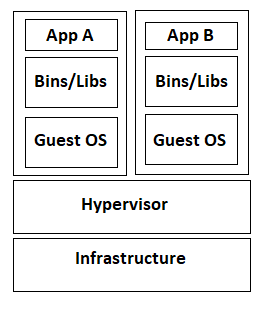
\includegraphics[width=0.5\textwidth]{Hypervisor.PNG}
  \caption[virtualization architecture]{virtualization architecture}
  \label{fig:virtualization architecture}
\end{figure}

\pagebreak Containerization, on the other hand, uses a different type of virtualization. In a containerization architecture there is no hypervisor, but a container engine which is situated on top of the operating system. This is beneficial as the operating system can no longer restrict certain applications from running. Containerization abstracts the underlying infrastructure by creating specific virtual pieces of the hardware infrastructure. This can be identified by image 2.2 below. The virtual aspects from the rest of the architecture are taken and create containers at the operating system level. When containerization is used, the operating system is the main feature and is shared among the containers. Whereas, in a virtualization architecture, the operating system is cloned for each virtual machine in the environment.

\begin{figure}[ht]
  \centering
      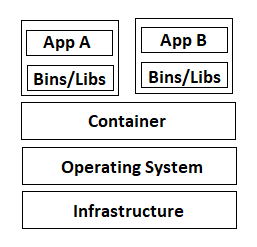
\includegraphics[width=0.5\textwidth]{Container.PNG}
  \caption[Containerization architecture]{Containerization architecture}
  \label{fig:Containerization architecture}
\end{figure}



\pagebreak As containerization essentially performs the virtualization of the operating system, this means that any type of compute device would be able to host a containerization platform. This is where single board computers come in. Single board computers as previously stated, are single circuit boards with microprocessors, memory, input/output and other aspects required to make a fully functioning computer.\cite{Reference17} There are many types of single board computers available if desired, throughout my time studying at Cork Institute of Technology I was exposed to two types of single board computers, Raspberry Pi's and Arduino's. A Raspberry Pi is a very popular single board computer which is used among schools and colleges to demonstrate how single board computers function. From figure 2.3 it can be seen that the Raspberry Pi is in fact a single switch board with all of the added commodities required by the user. One benefiting factor of this single board computer is the operating system element. A Raspberry Pi can a specialized Linux operating system, which, enables a user friendly environment.         


\begin{figure}[ht]
  \centering
      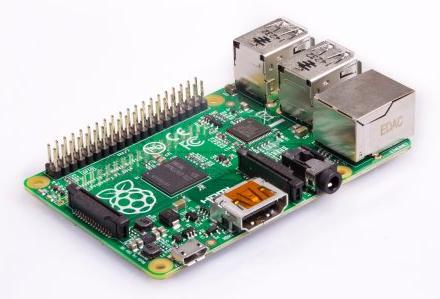
\includegraphics[width=0.7\textwidth]{RaspPi.PNG}
  \caption[RaspberryPi 2 Model]{RaspberryPi 2 Model \cite{Reference18}}
  \label{fig:RaspberryPi}
\end{figure}

\pagebreak The second single board computer which I will be researching for this project is an Arduino. Arduino is open-source, which is based off easy to use hardware and software. Arduino's function is by a micro-controller, this micro-controller can be sent any set of instructions that is to be executed. An Arduino can be used for a variety of things, depending on what the user desires. This element makes the Arduino appealing, but, Arduino's do not have their own operating system, meaning that the average user, with no programming knowledge would find it extremely difficult to benefit from the beauty of the Arduino.

\begin{figure}[ht]
  \centering
      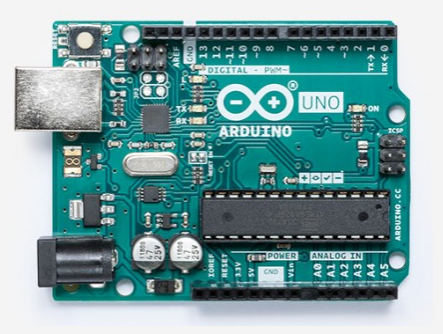
\includegraphics[width=0.7\textwidth]{Arduino.PNG}
  \caption[Arduino]{Arduino \cite{Reference19}}
  \label{fig:Arduino}
\end{figure}

\pagebreak Why single board computers? The decision to use single board computers throughout this project was adapted by a variety of reasons. They are inexpensive, open-source and easily usable. These aspects make this project achievable by anyone who would desire to re-create, while also helping to get the overall theory across as clearly and effectively as possible. These two types of single board computers are seen to be the most used in the world, meaning that users with any prior knowledge of computer science would know the functionality of these devices. For users who have no prior knowledge, the Raspberry Pi is a much more reactive single board computer. For this reason and for simplicity, two single board computers will be used throughout the implementation of this project. 

Single board computers are a necessity to achieve the desired outcome, but, the main reasoning behind choosing this topic was because of containerization. As containerization has been around for a long time but still quite unknown, I am going to delve into the area and outline every aspect of containerization.

\begin{itemize}
    \item What are containers?
    
    As previously stated containers are light weight software package that contains everything needed to run an application. More often than not, developers face issues when developing an application to ensure that it will be able to run on any device. To give an example of this, imagine having a mobile application, but it only being able to run on a Samsung phone but not an Apple device. Containers help to ensure that the application can be deployed anywhere. The functionality is, a container has a specialized environment which consists of all the underlying dependencies which would commonly be needed for development. On a higher level, libraries, binaries and configuration files (which can be seen from figure 2.2).
    
    \item Why containers?
    
    Containers are very lightweight, they can be only tens of megabytes in size in comparison to virtual machines. For this reason alone, containers are very appealing. Quick boot-up time is another huge benefit of containers. Having a quick boot-up time provides the application with almost instant run time, for instance, imagine having the option to have your laptop start-up and run straight away, or, needing to give it a few minutes to warm up before usage, having a quick start-up is always going to be the desired option. Finally, Containers and containerization, provides the opportunity to split all of the different aspects that an application would use to function into modules. This technique is also known as micro-services, another aspect of this project. Having the application split into modules allows for changes to be made much easier and conveniently, essentially, a developers dream. These modules can be installed and removed if required due to the light-weight architecture of containers.
    
    \item Types of containers
    
    The most popular container to date is Docker. Docker has single handily popularized container technologies over the last number of years. It has helped developers and corporations worldwide to understand that development and deployment can be made much simpler and more efficient. For this project, Docker is the container technology which I have chosen to be used as it is a Linux hosting container. But, there are many more container technologies that could be used. Tomcat, Jetty and Springboot are some examples of containers which are used by Java applications. Java containers are useful, but, Linux containers are going to be used for this specific project. Rocket containers or Rkt, was launched from CoreOS as a result of early security issues with Docker. These issues have been long been addresses, leaving Rkt behind. Even though there are these different types of containers, Docker is the one which is much more manageable.
    
    \item Docker
    
    Docker is an open-source container application which performs virtualization of the operating system in a virtual environment. It was designed and founded by Soloman Hykes, who is an engineer and now Chief Technology Officer of Docker. As previously stated, Docker is a Linux container but can also run on Windows OS and macOS. Dockers functionality is achieved by what are known as containers, these containers are run by a single operating system kernel ( a kernel is a computer program which controls every aspect of the system), which makes containerization much more lightweight than typical virtual machines.
    
    \item Managing Containers
    
    Like most things in technology, there is a level of management needed behind the scenes. Kubernetes is an open-source system for automating deployment , scaling and management of containerized applications. In other words, Kubernetes manages everything within a container. Kubernetes works extremely well with Docker, while Docker provides the container, Kubernetes orchestrates and manages the clusters of the container.  
    
    \item How does Kubernetes Work?
    
    Kubernetes is a platform for working with containers. It gives you the options to work with deployments, an easy way to scale and allows for monitoring. In Kubernetes, there is a master node which is used to create the container image you would prefer, this image then deploys and becomes the application. Kubernetes monitors of all of the applications which it has deployed, therefore, if an application were to go down, it tries to fix the issue and redeploy the application. In terms of scaling, Kubernetes will allow you to scale your application but will place the newly scaled deployment in a location which is determined by Kubernetes itself. This way, the resources are being used efficiently. 
    
\end{itemize}


%Position your topic within Computer Science. This activity will aid you in your literature review also. We zoom out to see three levels:

% notice the enumerate structure to create itemized lists
%\begin{enumerate}
   % \item What is the core topic your project is about? e.g., Mobile app for online voting. 
    %\item What core area(s) does the project fall under? e.g., Mobile applications, Social Networking, Service Providers. 
    %\item What main area(s) of Computer Science does the project fall under? e.g. Software Development, Cloud Computing.
%\end{enumerate}

%The ACM Computing Classification System (http://www.acm.org/about/class) will aid you in this, use the 2012 categories. Make sure to use figures and illustrations were appropriate. LaTeX will take care of the formatting of these. Do not try to get fancy here, you should concentrate on the content and not the formatting, this is why we are specifying LaTeX.

% Again take note of the structure, simply copy and paste this for future single figures


%You can specify the width and label for a figure which allows you to reference the figure and you can attribute a source in the figure caption as is done for figure \ref{fig:successkid}. Make sure you reference all external figures (i.e. figures you did not create yourself). Also use references for all figures e.g. use "... in figure \ref{fig:successkid} ..." NOT "... in the figure above ...".

%\section{Project Scope}
%Project specifics: Background minimum knowledge.

%Imagine you wanted to explain the specifics of your project to a person that knows nothing of Computer Science. You cannot talk about everything (as the idea is not to write a 500+ page report). Remember the reader at this stage can only be assumed to know what you have covered, so identify what are the minimum concepts belonging to the main areas (listed as 3 in the section before) and the core areas (listed as 2 in the section before) that you would need to explain so that the reader is able to understand the specifics of your project and indeed the following section. For example the minimum amount of knowledge about software development, cloud computing, mobile applications, social networking and service providers that are required so as to understand the specifics of a project about a mobile app for an on-line voting system. Here we are making the same trip we did before, but now in the opposite direction. Start zooming in from 3, then to 2 and finally to reach your project 1. Once the reader is finished this section they should be able to understand the proceeding sections (and have context for it within the project).


\section{A Review of Thematic Area}
During this section of the project, I will be displaying some of the resources that are available with regards to the topics I have and will be covering. Firstly, I will be discussing some of the conferences which are held all over the world on the topics of IOT, Cloud computing and containerization.

\begin{itemize}
    \item IEEE Global Conference on Internet of Things \cite{Reference2}
    
    IEEE stands for the Institute of Electrical and Electronics Engineers. This conference is held by the IEEE on the topic of Internet Of Things and its main goal is to provide a forum for innovation and research. This event is hosted annually at a range of different locations and provides keynote speakers from some of the top institutes in the world.
    
    \item Cloud Expo Europe \cite{Reference3}
    
    The Cloud Expo Europe conference dives into all aspects of cloud computing, including DevOps and infrastructure. As there are many aspects of cloud computing, this specific conference is divided up into specialized areas to ensure the attendies can get the full experience. These specialized ares include, Agile Networks, Fintech Finance and Banking Technology, Multi-Cloud strategy and management, and DevOps containers and open cloud. 
    
    \item KubeCon Europe \cite{Reference4}
    
    KubeCon Europe is run alongside KubeCon China and KubeCon North America. What makes KubeCon so appealing is that it focuses solely on Kubernetes and IOT, Micro-services and security for these aspects. It is also a Linux Foundation event which combines containerization and cloud computing communities together to hold open discussions. 
  
    
    \item DockerCon US and Europe \cite{Reference5}
    
    DockerCon is the most prestigious event of its kind. From its name, it is obvious who this conference is hosted by, Docker. Like other conferences, it offers a variety of panels with well known speakers and even workshops for its attendees. Anyone who uses docker or is interested in using docker attends this 3 day conference. 
    
    
    \item Cloud and DevOps World  \cite{Reference6}
    
    Cloud and DevOps world aims to delve into the world of cloud innovation. This includes containers and server-less architecture. It is a huge conference which is held in London annually and is hoping to change the future with cloud.
    
    
    
\end{itemize}


These conferences take place every year, proving that this area within computer science is very much relevant and constantly developing and improving. Along with these conferences, there are a number of books and journals written on the topics of Containerization, Single board computers and micro-services. 

\begin{itemize}
    \item \textit{Commodity single board computer cluster and their applications} \cite{Reference7}
    
    Commodity single board computer cluster and their applications is an article which is abstracted from volume 89 of the Future Generation Computer Systems journal. This journal covers all aspects of computer science and engineering. This article was released on the 30th of June 2018 and was written by a group of lecturers from universities around the United Kingdom. In short, this article dives into the area of single board computers specifically Raspberri Pi's along with the aspect of clustering SBC's. 
    
    \item \textit{Running Containers in Production} \cite{Reference8}
    
    This is a whitepaper which was released on the 19th of September 2018. The aim of this whitepaper is to explore the benefits of containers while also investigating the challenges that come with deploying containerized applications. The areas which are covered are building and managing container environments, monitoring and securing containers.
    
    \item \textit{The Docker Book} \cite{Reference9}
    
    Written by James Turnbull and released on the 4th of August 2014, The Docker Book containers everything one would need to know about the container Docker. Throughout this book, James writes in much detail about Docker along with every aspect that needs to be examined to understand containers and containerization applications.
    
\end{itemize}

There are many wikis, youtube videos and blogs regarding this area. I will list just some of these below:

\begin{itemize}
    \item Container Solutions \cite{Reference10}
    
    Container solutions is a blog which discusses all things container and containerization. Each blog post is written by a different individual who is an expert in this particular field. Container solutions has a huge following, with a newsletter emailed to those subscribed, there is no doubt container solutions will keep any individual up to date with all things containerization.
    
    \item Introduction to Micro-services, Docker and Kubernetes \cite{Reference11}
    
    This is a YouTube video which I found extremely helpful in the early stages of my research for this project. It explains in some detail the process of how Docker, Kubernetes and Micro-services coordinate and work together. The YouTube video was uploaded in November 2017 by James Quigley who has some videos regarding related topics. 
    
    \item Raspberry Pi Arduino Communication \cite{Reference12}
    
    Staying with YouTube videos, this video outlines how to connect Raspberry Pi's and Arduino's over a USB connection. This is extremely helpful to me as for this project, I will be attempting to migrate services between these two single board computers. The individual who is speaking explains in detail yet in a very understanding way the process of how to accomplish this communication. This YouTube video was uploaded by an account which is called nmBotTronics in January of 2016. 
    
    \item LoverPi \cite{Reference13}
    
    LoverPi is a website which is dedicated to all things Single board Computers. Not only is it a website which sells and distributes single board computers, but they also have a blog and wiki page dedicated solely to them. This is a one stop shop for everything related to SBC's.
    
    
    \item Degee U \cite{Reference14}
    
    Degee U is a YouTube channel run by DJ Spiess. DJ has been making videos on all topics related to programming, micro-services, Apache and many more for a number of years. One particular video which attracted me to his channel is his video titled "what are micro-services?". After watching this video I then found many other videos related to my topic of research from DJ and realized that his content would be of great use. 

    
\end{itemize}


As this project is based around the thematic area of Cloud Computing, HCI and Compute Systems, there are many companies worldwide who would design and implement what I hope to be the end product. Some of these companies include:

\begin{itemize}
    \item VMWare
    
    Is the leader in all things cloud infrastructure and virtual work-space technology. VMWare is known world wide for its ground breaking applications and infrastructure, their products are used by millions of customers in every corner of the world. 
    
    \item Google
    
    As a household name, every person to touch an online service has used Google's search engine. But, what many people who do not have the knowledge or an interest in the more in-depth aspect of this organization is, they have developed much more than just the Google search engine. Kubernetes was developed and founded by Joe Beda, Brendan Burns and Craig McLuckie. Once Google realized what Kubernetes was going to be, they sent two more engineers to ensure the application would be designed to its best ability. These two men were Brian Grant and Tim Hockin.
    
    \item Docker 
    
    Docker, as previously stated, is a container application which performs the virtualization of the operating system in a virtual environment. How Docker is going to be used in this project is unique as I will be installing Docker on single board computers, whereas Docker would typically be installed on much larger devices. 
    
\end{itemize}

%The focus of this section is at the heart of the project research phase. You must identify the main sources of information you should be aware of within your chosen area and pay regular attention to so as to strengthen your knowledge in the core topic you are working at. So here you should develop an knowledge of not only your core topic but also about the area of computer science the topic falls under. More specifically you should research the following:
%\begin{itemize}
   % \item The top 5 International Conferences and Journals most related to your topic. This is crucial, as it represents the main source for keeping you aware of what the state-of-the-art in your topic is.
  %  \begin{itemize}
        %\item In particular it will make you aware of what other projects related to yours have been already done (so that you can compare/position your project w.r.t. these).
        %\item What new techniques are being developed, so that you can apply them in your work. e.g. new frameworks for data visualization
  %  \end{itemize}
    %\item The top 3 most recent books/texts related to your topic. There are many free resources from which you may download a relevant text on the topic of your project. Try to either download or borrow 3 recent (no older than 10 years) texts relating to the topic your project is on which you will use throughout the project as reference material and to aid in tackling a number of the technical problems you may encounter. Any PhD/MSc thesis that have published in the last 5 years relating to the topic are also invaluable resources as they will contain a state of the art and references in your project topic. Approach these only after reading/viewing the wikis/Youtube videos you find as a certain level of knowledge will be assumed about the topic.
    %\item The top 5 companies/organizations potentially interested in the product you are developing. Finally, this is also crucial, as it forces you extend to purely programmer view of the project to a wider view considering the market, potential stakeholders and niches where your product can become useful. Moreover, Computer Science is a huge topic with loads of different works and roles. If you pick a project in the area you feel passionate about, and you identify what the market in this area is about, then you can drive your future professional career (from the very beginning) towards the path that makes you happier. I know that this does sound as a very technical reason, but I suppose we all agree is probably the most important of all reasons for choosing a particular project focus. 
    %\item The top 5 wiki/forums/blogs/Youtube channels most related to your topic. This is crucial to you as well, as it represents a more accessible, personal and less informal way of communication with people working/interested on the same topic as you are. This communication is extremely helpful for improving your skills, solving potential doubts and increase the interest/relevance of the topic/area itself.
%\end{itemize}

%You should begin your journey of discovery in reverse order to the listing above (which is given in order of academic importance/significance). So when you are researching your topic first look up some TedX talks or youtube tutorials, then research what companies are doing in the area, then get a handful of very good texts on the core topics of your area (anything older than 5 years usually is not helpful here) and finally start reading conference or journal papers (again newer is better here). In particular during this section you may need to use tables to list resources. These are also automatically formatted in latex thus allowing you to concentrate on content. for example table \ref{tab:Mylar}.

%\begin{table}[ht]
	%\centering
		%\begin{tabular}{ c  c  }
	%	\hline
	%	\hline
	%	Parameter & PET \\
	%	\hline
	%	Youngs Modulus & 2800-3100MPa \\
	%	Tensile Strength & 55-75MPa \\
	%	Glass Temperature & 75$^\circ$C \\
	%	Density & 1400kg/m$^3$ \\
	%	Thermal Conductivity & 0.15-0.24Wm$^{-1}$K$^{-1}$ \\
	%	Linear Expansion Coefficient & $7\times10^-5$ \\
	%	Relative Dielectric Constant @ 1MHz & 3\\
	%	Dielectric Breakdown Strength & 17kVmm$^{-1}$\\
	%	\end{tabular}
	%\caption{PET Physical Properties}
	%\label{tab:Mylar}
%\end{table}

To this current day, there has been much work performed in all of the areas this project falls under. One area in particular which has grown substantially in the last 10 years is Cloud Computing. When the term cloud computing first emerged back in the 2000's, people were confused as to what exactly it was. Now, the cloud is used in many ways and can be tailed to a specific need. In short, cloud computing can benefit organizations by minimizing their IT infrastructure costs. One main aspect of cloud computing is virtualization. Virtualization aims to speed up the operations in an organization while reducing costs, this is achieved by splitting physical components of a computing device into several virtual devices. These virtual devices can be easily managed and scaled, which is a characteristic that can be very appealing to growing corporations. There are many types of cloud computing or services available to its users.

\begin{itemize}
    \item \textit{Infrastructure as a Service (IaaS)}
    
    This service provides resources over the internet in a virtual manner. This model allows the cloud provider to host the fundamental assets of the infrastructure in an on-premise data centre. This allows for easier, faster and most importantly, a more cost effective operation of the underlying infrastructure. IaaS typically uses a management or orchestration technique to ensure that the virtual environment is run efficiently and to the highest standard.
    
    
    \item \textit{Platform as a Service (PaaS)}
    
    Platform as a service allows customers to manage, develop and run applications with ease. These customers would no longer be forced to worry about building complex infrastructures to develop and run such applications. Typically, this infrastructure is provided by a third party company who would allow access over the internet to such service. This is beneficial as having an underlying platform, which could include both hardware and software, to develop and run applications can be extremely costly. This cost is cut substantially if Platform as a service is implemented. A PaaS provider would analyze the situation and implement what they think is needed to ensure a business can perfrom the tasks required. 
    
    
    \item \textit{Software as a Service (SaaS)}
    
    SaaS provides the essential software that organizations would require. Third party companies provide applications to their customers over the internet. Usually, this would be at a fixed cost. For example, Cork Institute of Technology uses Gmail to host all of the email accounts for students and staff, this is a service which is provided over the internet to CIT. As a result, this removes the obligation of CIT to install a server to run this application, again, cutting costs. The ability to scale is a huge benefit of SaaS, again taking the email example from CIT, as more student enroll each year, more email addresses can be provided with much ease. 
    
\end{itemize}

Computing and Computer Science is changing rapidly, with new technologies being launched quicker than ever before. It is important to keep informed of these new trends and technologies. Two new technologies which have emerged recently are Edge Computing and Fog Computing. These technologies aim to ensure that the compute technologies involved in a network are functioning to the highest possible standard. This is achieved by working together and  pushing the huge amounts of data which is generated by IOT devices to different platforms which are one the edge of the network. 

\begin{itemize}
    \item Edge Computing
    
    Edge computing is exactly as it sounds. IOT devices can be referred to as edge devices. As we already know, single board computers are IOT devices as they generate their own data. Edge computing maintains all the data which was generated on it, while staying on the edge of the network. This is beneficial as it can help keep the network secure. 
    
    \item Fog Computing
    
    Fog computing is an architecture which is designed to connect cloud computing to the edge. Also referred to as the missing link in connecting and sending data to the cloud environment. Fog computing can be used to reduce bandwidth needed within network, as the devices are directly connected and data does not need to be sent back and forth between data centres. 
    
    
\end{itemize}

With the type of environment that will be created using single board computers to migrate micro-services, this could be considered a small fog/edge computing network. 

Complex Systems and Internet of Things are two areas which can be interlinked. There are studies which have occurred from many Universities on the topic of how IOT can help in managing complex systems. But what exactly is the Internet of Things? 

\begin{itemize}
    \item Internet of Things 
    
    The term internet of things evolved from Massachusetts Institute of Technology (MIT) in the late 1990's. Essentially, IOT is any device which can be interconnected. How these devices are connected comes from their ability to connect to the internet. Not only are these devices interconnected but they also collect and exchange data. Examples of IOT include, smart watches, smart phones and sensors, the list is endless and with new IOT devices being developed everyday, eventually everything will be classed as an IOT device. More recently, IOT devices allow freedom to its owners by acquiring the ability to be monitored and controlled from a remote location. Single board computers are classes as IOT devices as they can be interconnected and also have the ability to be connected to the internet and provide such data. 
    Data that is collected from IOT devices is being analyzed and examined by the creators. Like anything that is connected to the internet, data is generated and can be analyzed for research, used by businesses for analytics and/or to form a profile of you as a user. Some companies use this data to figure out what their next big strategic step would be.
\end{itemize}


%What has been done before in your community w.r.t. your topic? Once you have gotten an understanding of the topic and technologies and have identified the top 5 formal conferences/journals, wiki/forums/blogs/Youtube channels and companies/organizations the next step is to research in depth on them! And here in depth means in depth. Make sure you cite\cite{Reference1} a number of papers \cite{Reference3}, luckily Latex will take care of the ordering of the citations \cite{Reference2} for you.

%The aim here is that you find the trends in your topic (3), and more in general in the area in which your topic resides (2) your project falls under and from these trends you develop your initial project question further and begin to get insights into how others have solved/approached similar problems. Think of this section as colouring in your initial idea. Before you approach this section you should read at least 4/5 good literature reviews (a selection of last years projects will be posted on blackboard to aid you but you should find other sources also).

%In particular in this section, you must find and analyze at least 5 (ideally around 10) works belonging to, or at least related to, your work. You must describe these works and position your project w.r.t. them (i.e., clearly identify the similarities and differences between your project and each of these works). Also remember if you find that you are detailing topics that you have not introduced already here you need to add something to the earlier Scope section.